% ESE project report: College Support Assistant (RAG + LoRA/QLoRA fine-tuning)
% Build:  latexmk -pdf report.tex      (or run pdflatex twice so the index and figure numbers resolve)
% Screenshots go in images/ with the file names used in \screenshot{...} below.
% Until an image exists, a labelled placeholder box is printed in its place.

\documentclass[11pt,a4paper]{report}

\usepackage[margin=2.2cm]{geometry}
\usepackage[T1]{fontenc}
\usepackage{lmodern}
\usepackage{amsmath,amssymb}
\usepackage{graphicx}
\usepackage{booktabs}
\usepackage{tabularx}
\usepackage{array}
\usepackage{xcolor}
\usepackage{tikz}
\usetikzlibrary{arrows.meta,positioning,shapes.geometric,fit,calc}
\usepackage{pgfplots}
\pgfplotsset{compat=1.18}
\usepackage{float}
\usepackage{caption}
\usepackage{enumitem}
\usepackage{setspace}
\usepackage{titlesec}
\usepackage{etoolbox}
\usepackage[hidelinks]{hyperref}

\setstretch{1.2}
\setlength{\emergencystretch}{2em}
% chapters continue on the same page instead of starting a new one
\makeatletter\patchcmd{\chapter}{\if@openright\cleardoublepage\else\clearpage\fi}{\par\vspace{6pt}}{}{}\makeatother
\setlist{itemsep=2pt,topsep=4pt}
\titleformat{\chapter}[hang]{\Large\bfseries}{\thechapter.}{0.6em}{}
\titlespacing*{\chapter}{0pt}{10pt}{8pt}
\graphicspath{{images/}}

\newcommand{\repourl}{\url{https://github.com/Dcode-7/LLM_Mini_Project}}

% ---------------------------------------------------------------- diagram shades (black and white only)
\colorlet{accent}{black}
\colorlet{accentlight}{white}
\colorlet{warm}{black}
\colorlet{warmlight}{black!12}
\colorlet{greylight}{black!4}

\tikzset{
  box/.style={draw=accent, fill=accentlight, rounded corners=3pt, align=center,
              font=\small, minimum height=9mm, inner sep=4pt, text width=#1},
  box/.default=3.2cm,
  altbox/.style={box=#1, draw=warm, fill=warmlight},
  altbox/.default=3.2cm,
  plain/.style={draw=black!45, fill=greylight, rounded corners=3pt, align=center,
                font=\small, minimum height=9mm, inner sep=4pt, text width=#1},
  plain/.default=3.2cm,
  decision/.style={diamond, aspect=2.4, draw=warm, fill=warmlight, align=center,
                   font=\small, inner sep=1pt},
  flow/.style={-{Stealth[length=2.6mm]}, thick, draw=black!70},
  note/.style={font=\footnotesize\itshape, text=black!65, align=center},
}

% \screenshot[max height]{file}{caption}{label}{what to capture}: the image if present, otherwise a placeholder.
% Placed exactly where it appears in the text ([H]) so floats never split the surrounding sections.
\newcommand{\screenshot}[5][0.23]{%
  \begin{figure}[H]
    \centering
    \IfFileExists{images/#2}{%
      \fbox{\includegraphics[width=0.95\linewidth,height=#1\textheight,keepaspectratio]{#2}}%
    }{%
      \fbox{\parbox[c][#1\textheight][c]{0.88\linewidth}{\centering
        \textbf{\large Screenshot to add}\\[4pt]
        \texttt{images/\detokenize{#2}}\\[8pt]
        \parbox{0.85\linewidth}{\centering\small #5}}}%
    }
    \caption{#3}\label{#4}
  \end{figure}}

\begin{document}

% ================================================================= 1. TITLE PAGE
\begin{titlepage}
\vspace*{0.025cm}
{\centering
{\Large\textbf {RAG-based College Support Assistant}}\\
\vspace{0.55cm}
submitted in partial fulfillment of the requirement\\
for the award of the Degree of\\\vspace{0.65cm}
{\large\textbf {Bachelor of Technology}}\\
in \\
{\large\textbf {Computer Engineering}}\\
\vspace{0.50cm}
by\\
\vspace{0.55cm}
{\large \textbf {Divya Kumaar}}\\
\vspace{1.2cm}
% logo: spitlogo.pdf (or .png) in report/ or report/images/
\IfFileExists{spitlogo.pdf}{\includegraphics[scale=0.7]{spitlogo.pdf}\\}{%
\IfFileExists{images/spitlogo.pdf}{\includegraphics[scale=0.7]{spitlogo.pdf}\\}{%
\IfFileExists{spitlogo.png}{\includegraphics[width=4cm]{spitlogo.png}\\}{%
\IfFileExists{images/spitlogo.png}{\includegraphics[width=4cm]{spitlogo.png}\\}{}}}}
\vspace{0.8cm}
\textbf{Department of Computer Engineering}\\
Bharatiya  Vidya Bhavan's\\
Sardar Patel Institute of Technology\\
(Autonomous Institute Affiliated to University of Mumbai)\\
Munshi Nagar, Andheri-West, Mumbai-400058\\
University of Mumbai\\
\vfill
2026-2027\par}
\end{titlepage}


% ================================================================= 2. INDEX
\pagenumbering{roman}
\renewcommand{\contentsname}{Index}
\tableofcontents
\clearpage
\pagenumbering{arabic}

% ================================================================= 3. ABSTRACT
\chapter*{Abstract}
\addcontentsline{toc}{chapter}{Abstract}

Students ask a college helpdesk the same questions every year: fees, exam forms, hostel rules,
certificates and scholarships. The answers already exist in handbooks, but finding them is slow
and the student is often unsure which office to approach. This project builds a
\textbf{College Support Assistant} that answers such questions from the college's own handbook
and, for every answer, also raises a helpdesk ticket naming the responsible department, the
category, the priority and the next action.

The assistant uses \textbf{Retrieval-Augmented Generation (RAG)}. A 23-page Student Helpdesk
Handbook (PDF) is extracted, cleaned and split into 121 topic-level chunks with metadata. A hybrid
word and character TF-IDF retriever selects the three most relevant chunks, and a similarity
threshold makes the assistant refuse questions the handbook does not cover instead of inventing
an answer. The language model behind the answers is swappable: a cloud API, a local Ollama model,
an extractive (no-LLM) mode, or our own fine-tuned model.

For the fine-tuned model, \textbf{Qwen2.5-0.5B-Instruct} was adapted with \textbf{LoRA} and
\textbf{QLoRA}, training only 4.40\,M of its 494\,M parameters (0.89\,\%). On held-out
paraphrased questions, answer word-overlap F1 rose from 0.523 for the base model to 0.962 (LoRA)
and 0.975 (QLoRA), and the share of exact facts reproduced rose from 51\,\% to 97--98\,\%.
QLoRA's 4-bit base reduced peak training memory from 9.3\,GB to 5.4\,GB, which fits the 6\,GB
laptop GPU used. The system is delivered as a Streamlit web app (deployed on Streamlit Community
Cloud) and a FastAPI REST service, with input validation, rate limiting, logging, latency
measurement and 30 automated tests.

\medskip
\noindent\textbf{Keywords:} Retrieval-Augmented Generation, LoRA, QLoRA, parameter-efficient
fine-tuning, TF-IDF retrieval, Streamlit, FastAPI, helpdesk automation.

% ================================================================= 4. INTRODUCTION
\chapter{Introduction}

\section{Problem statement}
A college helpdesk receives a large volume of repetitive queries. Each one costs staff time, and
students wait for answers that are already written down somewhere. A plain chatbot built on a
general-purpose LLM is not a safe replacement: the model does not know the college's fees,
deadlines or contacts, and it may confidently invent them. The helpdesk also needs more than an
answer. It needs to know which office should handle the request and how urgent it is.

\section{Objectives}
\begin{enumerate}
  \item Answer student questions using only the college's official handbook, with the source page
        shown for every answer.
  \item Refuse questions the handbook does not cover, and direct the student to a human contact.
  \item Route every query by generating a ticket: department, category, priority and action.
  \item Fine-tune a small open model with LoRA and QLoRA so that it answers in the college's exact
        wording, and compare it with the base model.
  \item Deliver the system as a hosted web app and a REST API with validation, error handling,
        logging, response-time measurement and tests.
\end{enumerate}

\section{Scope}
The knowledge base is a \emph{Student Helpdesk Handbook} for \emph{Northbridge College of
Engineering \& Technology}, a fictional sample institution. It has 15 sections (Admissions, Fees,
Scholarships, Examinations, Academics, Library, Hostel, Placements, IT Services, Transport,
Certificates, Student Welfare, Medical, Sports and Clubs, General Information) and 121 topics.
Replacing the PDF with a real college's handbook in the same layout is enough to adapt the system.

\section{Technologies used}
\texttt{pypdf} and \texttt{reportlab} (PDF), \texttt{scikit-learn} TF-IDF (retrieval), an
OpenAI-compatible cloud API (Groq), Ollama, and Hugging Face \texttt{transformers}, \texttt{peft} and
\texttt{bitsandbytes} with PyTorch (LLMs and fine-tuning), Streamlit and FastAPI with Pydantic
(interfaces), \texttt{pytest} (testing), GitHub and Streamlit Community Cloud (hosting).

\section{Project repository}
The source code, handbook PDF, fine-tuning scripts, results and tests are available on GitHub at
\repourl.


% ================================================================= 5. APPLICATION WORKFLOW
\chapter{Application Workflow}

\section{System architecture}
Figure~\ref{fig:arch} shows the complete system. The handbook is processed once at startup; each
question then passes through validation, retrieval and an LLM backend before the answer and ticket
are returned to the user.

\begin{figure}[H]
\centering
\resizebox{0.6\linewidth}{!}{%
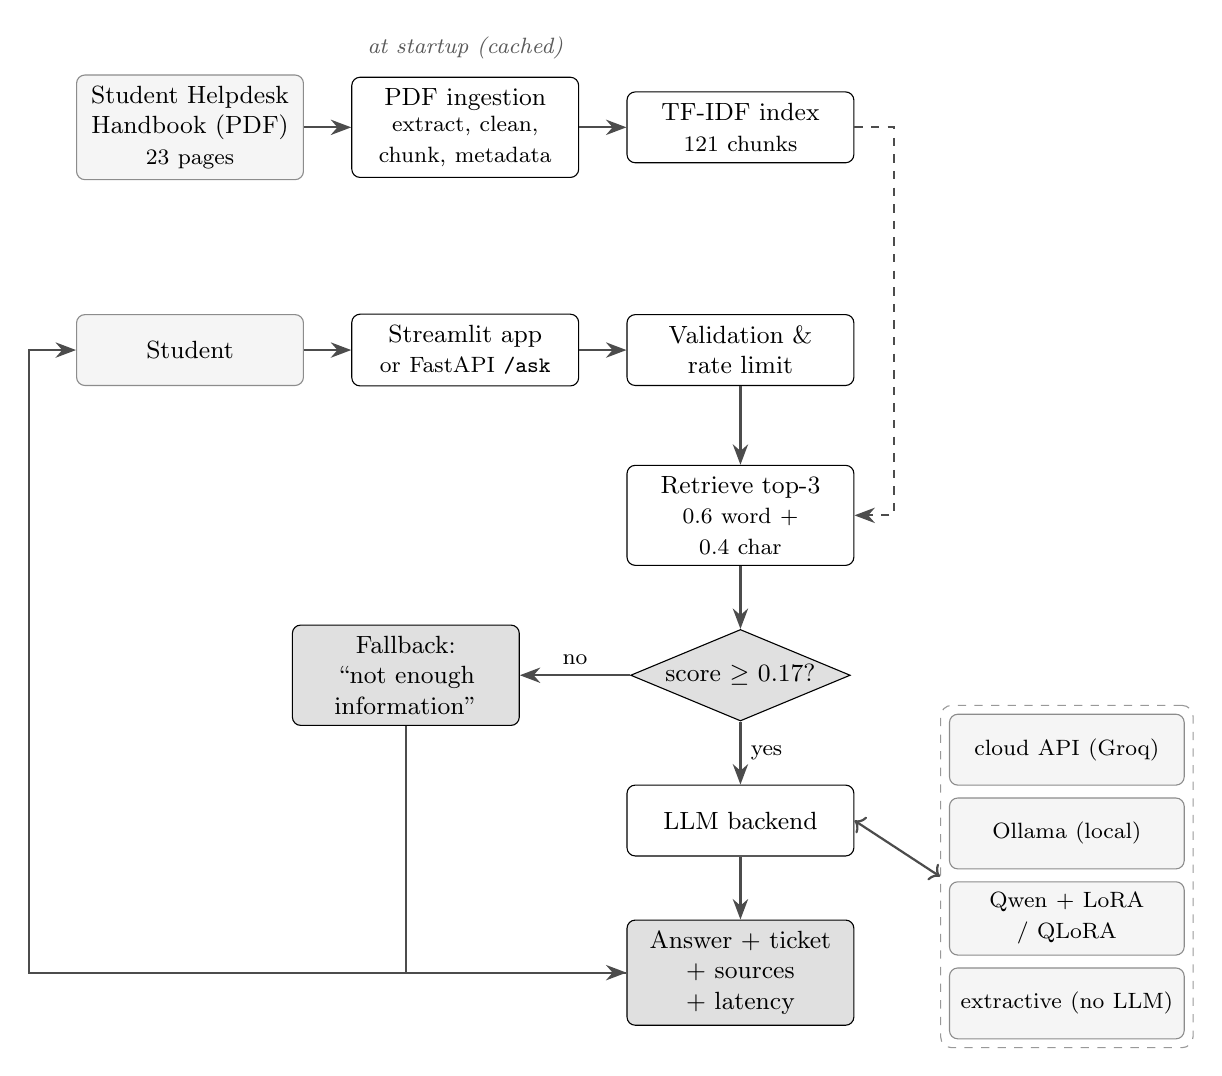
\begin{tikzpicture}[node distance=7mm and 6mm]
  % offline / startup lane
  \node[plain=2.6cm] (pdf) {Student Helpdesk\\Handbook (PDF)\\\footnotesize 23 pages};
  \node[box=2.6cm, right=of pdf] (ingest) {PDF ingestion\\\footnotesize extract, clean,\\chunk, metadata};
  \node[box=2.6cm, right=of ingest] (index) {TF-IDF index\\\footnotesize 121 chunks};
  \node[note, above=1mm of ingest] {at startup (cached)};

  % users
  \node[plain=2.6cm, below=17mm of pdf] (user) {Student};
  \node[box=2.6cm, right=of user] (ui) {Streamlit app\\\footnotesize or FastAPI \texttt{/ask}};
  \node[box=2.6cm, right=of ui] (val) {Validation \&\\rate limit};

  % pipeline
  \node[box=2.6cm, below=10mm of val] (ret) {Retrieve top-3\\\footnotesize 0.6 word + 0.4 char};
  \node[decision, below=8mm of ret] (thr) {score $\geq$ 0.17?};
  \node[altbox=2.6cm, left=14mm of thr] (fb) {Fallback:\\``not enough\\information''};
  \node[box=2.6cm, below=8mm of thr] (llm) {LLM backend};
  \node[altbox=2.6cm, below=8mm of llm] (out) {Answer + ticket\\+ sources + latency};

  % backends
  \node[plain=2.7cm, right=12mm of llm, yshift=9mm] (b1) {\footnotesize cloud API (Groq)};
  \node[plain=2.7cm, below=1.5mm of b1] (b2) {\footnotesize Ollama (local)};
  \node[plain=2.7cm, below=1.5mm of b2] (b3) {\footnotesize Qwen + LoRA / QLoRA};
  \node[plain=2.7cm, below=1.5mm of b3] (b4) {\footnotesize extractive (no LLM)};
  \node[draw=black!40, dashed, rounded corners, fit=(b1)(b4), inner sep=3pt] (bk) {};

  \draw[flow] (pdf) -- (ingest);
  \draw[flow] (ingest) -- (index);
  \draw[flow] (user) -- (ui);
  \draw[flow] (ui) -- (val);
  \draw[flow] (val) -- (ret);
  \draw[flow, dashed] (index.east) -- ++(5mm,0) |- (ret.east);
  \draw[flow] (ret) -- (thr);
  \draw[flow] (thr) -- node[right,font=\footnotesize]{yes} (llm);
  \draw[flow] (thr) -- node[above,font=\footnotesize]{no} (fb);
  \draw[flow] (llm) -- (out);
  \draw[flow, <->] (llm.east) -- (bk.west);
  \draw[flow] (fb.south) |- (out.west);
  \draw[flow] (out.west) -| ([xshift=-6mm]user.south west) |- (user.west);
\end{tikzpicture}}
\caption{System architecture}\label{fig:arch}
\end{figure}

\section{Knowledge base: from PDF to chunks}
The handbook is the only source of knowledge. Figure~\ref{fig:ingest} shows how
\texttt{pdf\_ingest.py} turns it into retrievable chunks.

\begin{figure}[H]
\centering
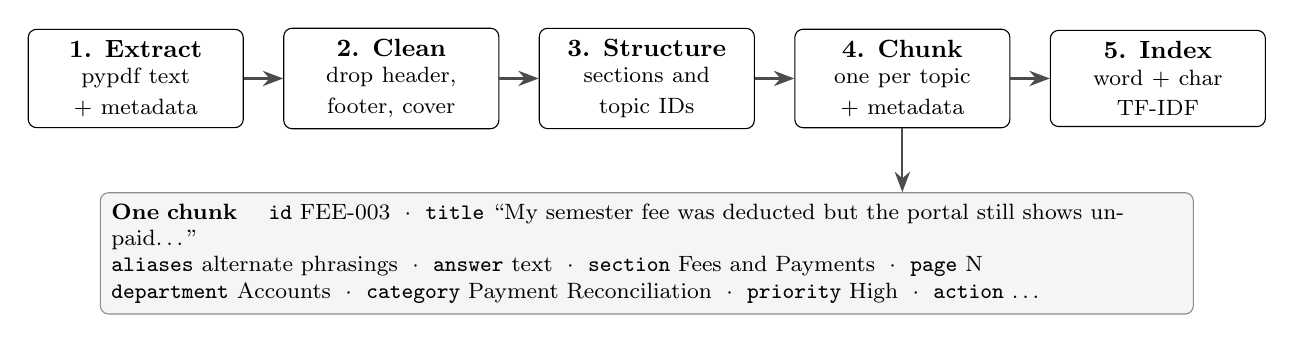
\begin{tikzpicture}[node distance=5mm]
  \node[box=2.45cm] (s1) {\textbf{1. Extract}\\\footnotesize pypdf text\\+ metadata};
  \node[box=2.45cm, right=of s1] (s2) {\textbf{2. Clean}\\\footnotesize drop header,\\footer, cover};
  \node[box=2.45cm, right=of s2] (s3) {\textbf{3. Structure}\\\footnotesize sections and\\topic IDs};
  \node[box=2.45cm, right=of s3] (s4) {\textbf{4. Chunk}\\\footnotesize one per topic\\+ metadata};
  \node[box=2.45cm, right=of s4] (s5) {\textbf{5. Index}\\\footnotesize word + char\\TF-IDF};
  \foreach \a/\b in {s1/s2,s2/s3,s3/s4,s4/s5} \draw[flow] (\a) -- (\b);

  \node[plain=13.6cm, below=8mm of s3, align=left, font=\footnotesize] (chunk) {%
    \textbf{One chunk} \quad
    \texttt{id} FEE-003 \;$\cdot$\; \texttt{title} ``My semester fee was deducted but the portal still shows unpaid\dots''\\
    \texttt{aliases} alternate phrasings \;$\cdot$\; \texttt{answer} text \;$\cdot$\; \texttt{section} Fees and Payments \;$\cdot$\; \texttt{page} N\\
    \texttt{department} Accounts \;$\cdot$\; \texttt{category} Payment Reconciliation \;$\cdot$\; \texttt{priority} High \;$\cdot$\; \texttt{action} \dots};
  \draw[flow] (s4.south) -- (s4.south |- chunk.north);
\end{tikzpicture}
\caption{PDF ingestion pipeline and the fields stored with each chunk}\label{fig:ingest}
\end{figure}

On the handbook this gives 23 pages extracted, three header and footer lines removed per page,
the cover and contents pages discarded, 15 sections and 121 topics detected, and 121 chunks of
190--452 characters. Answers longer than 900 characters would be split with a 150-character overlap.

\noindent\textbf{Why chunk by structure and not by size?} Splitting the same text every 500
characters would cut across topics, so a chunk could hold the end of one policy and the start of
another, and the routing line could be separated from its answer. Chunking at topic boundaries
keeps every answer whole and its ticket fields attached.

\section{Question answering flow}
\begin{enumerate}
  \item \textbf{Validation.} The question must not be blank and must be at most 1000 characters.
        Each session may ask at most 30 questions per minute.
  \item \textbf{Retrieval.} The question is scored against every chunk with
        $\text{score} = 0.6\cdot\cos_{\text{word}} + 0.4\cdot\cos_{\text{char}}$. Word n-grams
        match vocabulary; character n-grams tolerate typos and word variants (``fee'', ``fees'').
  \item \textbf{Threshold.} If the best score is below 0.17, the assistant replies that it does
        not have enough information and gives the front-office contact. No LLM call is made.
  \item \textbf{Generation.} Otherwise the top three chunks are placed in the prompt and sent to
        the selected backend, which must answer only from that context.
  \item \textbf{Response.} The answer is returned with a \emph{grounded} flag, the ticket from the
        best chunk's metadata, the source topics with page numbers, and the response time.
\end{enumerate}

\section{Fine-tuning workflow}
\begin{figure}[H]
\centering
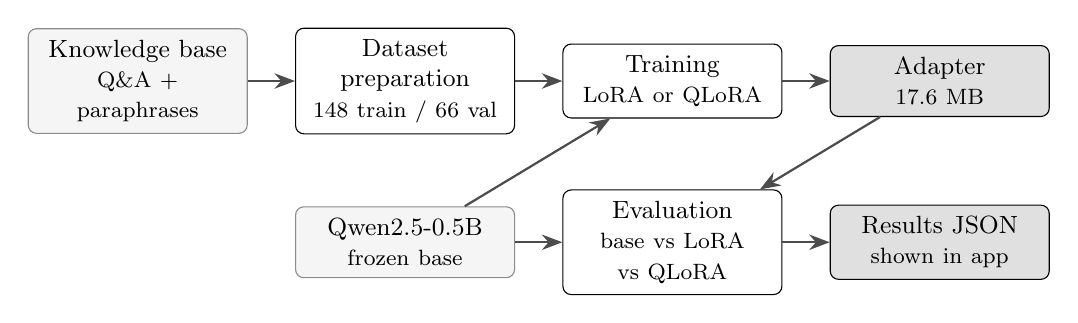
\begin{tikzpicture}[node distance=6mm]
  \node[plain=2.5cm] (kb) {Knowledge base\\\footnotesize Q\&A + paraphrases};
  \node[box=2.5cm, right=of kb] (prep) {Dataset preparation\\\footnotesize 148 train / 66 val};
  \node[box=2.5cm, right=of prep] (train) {Training\\\footnotesize LoRA or QLoRA};
  \node[altbox=2.5cm, right=of train] (ad) {Adapter\\\footnotesize 17.6 MB};
  \node[box=2.5cm, below=9mm of train] (eval) {Evaluation\\\footnotesize base vs LoRA vs QLoRA};
  \node[plain=2.5cm, left=of eval] (base) {Qwen2.5-0.5B\\\footnotesize frozen base};
  \node[altbox=2.5cm, right=of eval] (res) {Results JSON\\\footnotesize shown in app};
  \draw[flow] (kb) -- (prep);
  \draw[flow] (prep) -- (train);
  \draw[flow] (train) -- (ad);
  \draw[flow] (base) -- (train);
  \draw[flow] (ad) -- (eval);
  \draw[flow] (base) -- (eval);
  \draw[flow] (eval) -- (res);
\end{tikzpicture}
\caption{Fine-tuning workflow}\label{fig:ftflow}
\end{figure}

Every training example uses the same retrieved-context prompt as the app. The model is trained on
the canonical question and its paraphrases; one paraphrase per topic is held out for validation,
together with off-topic questions that must be refused.

\paragraph{How LoRA works.} The pretrained weight matrix $W_0$ is frozen. A trainable low-rank
update $\Delta W = BA$ is added beside it, so the layer computes $h = W_0x + \frac{\alpha}{r}BAx$.
With $W_0 \in \mathbb{R}^{d\times k}$, $B \in \mathbb{R}^{d\times r}$ and
$A \in \mathbb{R}^{r\times k}$, only $r(d+k)$ parameters are trained instead of $dk$. For a
$4096\times4096$ matrix with $r=8$ that is 256 times fewer. \textbf{QLoRA} stores the frozen base
in 4-bit NF4 with double quantisation and computes in bfloat16, and uses a paged 8-bit optimiser.

\begin{figure}[H]
\centering
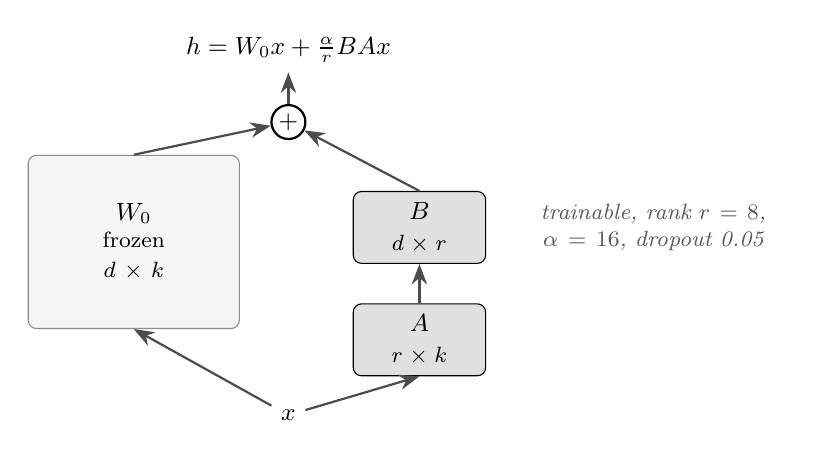
\begin{tikzpicture}[node distance=4mm]
  \node[font=\small] (x) {$x$};
  \node[plain=2.4cm, above left=9mm and 4mm of x, minimum height=2.2cm] (w0) {$W_0$\\\footnotesize frozen\\$d\times k$};
  \node[altbox=1.4cm, above right=3mm and 6mm of x] (a) {$A$\\\footnotesize $r\times k$};
  \node[altbox=1.4cm, above=5mm of a] (b) {$B$\\\footnotesize $d\times r$};
  \node[circle, draw, thick, inner sep=1pt, above=33mm of x, font=\small] (plus) {$+$};
  \node[font=\small, above=4mm of plus] (h) {$h = W_0x + \tfrac{\alpha}{r}BAx$};
  \draw[flow] (x) -- (w0.south);
  \draw[flow] (x) -- (a.south);
  \draw[flow] (a) -- (b);
  \draw[flow] (w0.north) -- (plus);
  \draw[flow] (b.north) -- (plus);
  \draw[flow] (plus) -- (h);
  \node[note, right=3mm of b, text width=3.4cm] {trainable, rank $r = 8$,\\$\alpha = 16$, dropout 0.05};
\end{tikzpicture}
\caption{A LoRA layer: frozen base weights plus a trainable low-rank update}\label{fig:lora}
\end{figure}

\noindent\textbf{Configuration.} Base model Qwen/Qwen2.5-0.5B-Instruct (494\,M parameters); LoRA on
\texttt{q,k,v,o\_proj} and \texttt{gate,up,down\_proj} with $r=8$, $\alpha=16$, dropout 0.05; 3 epochs,
learning rate $2\times10^{-4}$, batch size 4 with gradient accumulation 2; trained on an NVIDIA
RTX 3050 6\,GB laptop GPU.

\section{Application screens}
The Streamlit app has three pages: the Assistant, the Knowledge base (PDF) page, and the
Fine-tuning page. The FastAPI service exposes the same pipeline as a REST API.


\screenshot[0.2]{ss_answer_ticket.png}{Answer with helpdesk ticket and sources}{fig:ss-answer}
  {Ask ``My semester fee was deducted but the portal still shows unpaid''. Capture the answer,
   the ticket box (Department, Priority, Category, Action), the caption line with the response
   time, and the Sources expander opened.}

\screenshot[0.2]{ss_kb_page.png}{Knowledge base page: source document and pipeline}{fig:ss-kb}
  {Knowledge base (PDF) page, top part: Pages 23, File size, Sections 15, Chunks indexed 121,
   and the processing pipeline below it.}


\screenshot{ss_fastapi_docs.png}{FastAPI interactive documentation}{fig:ss-docs}
  {Run \texttt{uvicorn app:app} and open \texttt{http://127.0.0.1:8000/docs}. Expand
   \texttt{POST /ask}, click ``Try it out'', send a question and capture the JSON response.}

% ================================================================= 6. RESULTS / OBSERVATIONS
\chapter{Results and Observations}

\section{Functional test observations}
Table~\ref{tab:obs} lists the test cases run against the application with the extractive
backend. All seven passed. The project also has 30 automated \texttt{pytest} tests covering PDF
ingestion, the API endpoints and the Streamlit pages.

\begin{table}[H]
  \centering
  \caption{Observation table}\label{tab:obs}
  \small
  \begin{tabularx}{\linewidth}{>{\raggedright}p{2.7cm} >{\raggedright}p{2.8cm} X c}
    \toprule
    Test case & Expected result & Actual result & Result \\
    \midrule
    Health endpoint & API reports running & \texttt{200}, status ok, backend extractive, 121 KB entries & Pass \\
    Supported question & Grounded answer & ``lost library book'' $\rightarrow$ LIB-003 answer, ticket Library / Medium & Pass \\
    Unsupported question & Fallback message & ``capital of Australia'' $\rightarrow$ fallback, grounded = false & Pass \\
    Empty question & Validation error & \texttt{422} ``Question must not be empty''; Streamlit shows a warning & Pass \\
    Too-long question & Rejected & 1001 characters $\rightarrow$ \texttt{422} ``too long (maximum 1000 characters)'' & Pass \\
    Backend unavailable & Controlled error, no secrets & \texttt{503} backend\_unavailable; reason logged server-side only & Pass \\
    Response time & Latency recorded & \texttt{latency\_ms} in every response and log line ($\approx$4\,ms extractive) & Pass \\
    \bottomrule
  \end{tabularx}
\end{table}

\screenshot{ss_fallback.png}{Out-of-scope question is refused}{fig:ss-fallback}
  {Ask ``What is the capital of Australia?'' and capture the fallback answer with
   ``not in knowledge base'' in the caption line.}


\section{Training results}
\begin{table}[H]
  \centering
  \caption{LoRA and QLoRA training results}\label{tab:train}
  \begin{tabular}{lcc}
    \toprule
                                 & LoRA & QLoRA \\
    \midrule
    Frozen base stored as        & bfloat16 & 4-bit NF4 + double quant \\
    Trainable parameters         & 4.40\,M (0.89\,\%) & 4.40\,M (0.89\,\%) \\
    Base-weight memory           & 988\,MB & 724\,MB \\
    Peak GPU memory (training)   & 9.3\,GB & \textbf{5.4\,GB} \\
    Training time                & 201\,s & 191\,s \\
    Final validation loss        & \textbf{0.043} & 0.048 \\
    Saved adapter size           & 17.6\,MB & 17.6\,MB \\
    \bottomrule
  \end{tabular}
\end{table}

\screenshot{ss_training_loss.png}{Training loss per step, LoRA and QLoRA, 3 epochs}{fig:loss}
  {Fine-tuning (LoRA / QLoRA) page, section ``3 $\cdot$ Training loss'': the line chart with
   the LoRA and QLoRA curves and its legend.}

\noindent Validation loss after epochs 1, 2 and 3 was 0.045, 0.043 and 0.043 for LoRA, and
0.051, 0.048 and 0.048 for QLoRA. Both curves flatten after the second epoch, so three epochs
were enough.

\section{Evaluation on held-out questions}
The validation set has 66 questions: 63 paraphrases never seen in training and 3 new off-topic
questions. Every model received the same retrieved context and used greedy decoding.
Figure~\ref{fig:eval} shows the results: answer F1 was 0.523 for the base model, 0.962 with LoRA
and 0.975 with QLoRA; facts reproduced were 51\,\%, 97\,\% and 98\,\%; off-topic questions refused
were 3/3, 3/3 and 2/3; and generation took 2.5, 8.2 and 9.7\,s per answer.

\screenshot{ss_eval_table.png}{Evaluation of the base and fine-tuned models}{fig:eval}
  {Fine-tuning (LoRA / QLoRA) page, section ``4 $\cdot$ Does fine-tuning help?'': the table
   with Base, Base + LoRA and Base + QLoRA columns.}

\screenshot[0.3]{ss_finetuning_page.png}{LoRA vs QLoRA comparison in the app}{fig:ss-ft}
  {Fine-tuning (LoRA / QLoRA) page, section ``2 $\cdot$ LoRA vs QLoRA'': the table with the
   LoRA and QLoRA columns (memory, rank, training time, validation loss, adapter size).}

\section{Observations}
\begin{enumerate}
  \item \textbf{Fine-tuning changed the behaviour, not the knowledge.} With the same context, the
        base model often rambled or dropped details: asked about going home from the hostel, it
        returned only the sentence on late entry, while both adapters gave the full leave procedure.
        Both adapters
        reproduced the college's exact answer, raising answer F1 from 0.52 to over 0.96.
  \item \textbf{Under 1\,\% of the parameters were enough.} Only 4.40\,M of 494\,M parameters
        were trained, and the saved adapter is 17.6\,MB. The full base model is still needed at
        inference.
  \item \textbf{Weight size is not training memory.} The bf16 weights take about 1\,GB, but LoRA
        training peaked at 9.3\,GB because of activations, gradients and optimiser state, and
        spilled past the 6\,GB VRAM into shared memory.
  \item \textbf{QLoRA made training fit the GPU.} The 4-bit base brought the peak to 5.4\,GB at
        almost the same validation loss (0.048 vs 0.043). The base is 724\,MB rather than about
        250\,MB because embeddings and the output layer stay unquantised.
  \item \textbf{QLoRA missed one refusal.} For ``Recommend a good movie'' it answered with the mess
        feedback topic. Three off-topic questions is a small sample; more refusal examples should
        be added to training before relying on it.
  \item \textbf{LoRA did not make inference faster.} The unmerged adapter adds extra matrix
        multiplications, the fine-tuned answers are longer because they are complete, and the
        4-bit base is dequantised on the fly.
  \item \textbf{The threshold prevents invented answers.} Questions outside the handbook score
        below 0.17 and get the fallback message without any LLM call.
  \item \textbf{Scores are helped by retrieval.} The evaluation scores are high partly because the
        retriever already puts the right topic in the prompt; the adapter learned to use that
        context faithfully, which is the intended division of work between RAG and LoRA.
\end{enumerate}

\screenshot{ss_deployed.png}{Application deployed on Streamlit Community Cloud}{fig:ss-cloud}
  {The live app in the browser with its \texttt{*.streamlit.app} address visible in the address
   bar, showing an answered question.}

% ================================================================= 7. CONCLUSION
\chapter{Conclusion}

This project built a College Support Assistant that answers student questions from the college's
own handbook and routes every query to the right office with a ticket. Processing the handbook PDF
into topic-level chunks kept each answer intact with its routing details, and the similarity
threshold made the assistant say ``I don't know'' rather than invent college policies.

Fine-tuning Qwen2.5-0.5B-Instruct with LoRA and QLoRA showed that parameter-efficient methods can
adapt a model on a 6\,GB laptop GPU: training under 1\,\% of the parameters raised answer F1 from
0.52 to above 0.96 and fact accuracy from 51\,\% to 97--98\,\%. QLoRA matched LoRA's accuracy while
cutting peak training memory from 9.3\,GB to 5.4\,GB. Combining the two approaches worked as
intended: RAG keeps the knowledge current without retraining, and the adapter makes the model use
that knowledge precisely.

The system is available as a hosted Streamlit app and a FastAPI service with validation, rate
limiting, logging, latency measurement and automated tests.

\section{Limitations}
\begin{itemize}
  \item The handbook and all its data are fictional sample data.
  \item TF-IDF retrieval matches words, not meaning; a question phrased very differently from the
        handbook may score below the threshold.
  \item The fine-tuned models were trained on the original 63 topics; the 58 topics added later
        are answered through retrieval but were not part of fine-tuning.
  \item The hosted app has no GPU, so it uses a cloud API or the extractive backend; the fine-tuned
        model runs locally.
\end{itemize}

\section{Future scope}
\begin{itemize}
  \item Use dense embeddings (or a hybrid with TF-IDF) and a re-ranker for semantic retrieval.
  \item Retrain the adapters on all 121 topics with more off-topic refusal examples.
  \item Send tickets to a real helpdesk system and notify the responsible department.
  \item Add student login, multilingual support (Hindi, Marathi) and conversation memory.
  \item For production: authentication, HTTPS, monitoring and managed secrets.
\end{itemize}

\end{document}
